\documentclass[
	11pt, 
	DIV10,
	ngerman,
	a4paper, 
	oneside, 
	headings=normal, 
	captions=tableheading,
	final, 
	numbers=noenddot
]{scrartcl}


\usepackage[ruled]{algorithm2e}
\usepackage{graphicx}
\usepackage{hyperref}
\usepackage{amsmath}
\usepackage{mathtools}
\DeclarePairedDelimiter{\ceil}{\lceil}{\rceil}
\DeclarePairedDelimiter{\norm}{\lVert}{\rVert}

\title{An Implementation of SPH-based Solvers for Fluid Simulation}
\author{Yinglun, Qihui, Iohannes}

\begin{document}
\maketitle


\section{Motivation}

In this work, we follow the basic principles of smoothed particle hydrodynamics (SPH) to implement two of the most classic approaches in fluid simulation. We carry out extensive studies on the behavior of fluid particles under varying experimental conditions, as well as provide a handful of insights on the reason behind certain fluid behaviours in general. The rest of this report will be divided into three sections. In section \ref{sec2}, we explain how we setup the scene, how we choose to design the simulation pipeline and how the fundamentals of SPH-based simulation work in our implementation; in section \ref{sec3}, we discuss how particle accelerations are computed in a weakly compressible SPH solver and how an iterative procedure can be implemented to model position-based fluids; in the last section \ref{sec4}, we conduct control experiments under various simulation conditions and test scenes to showcase how the different hyperparams affect the behavior of the fluid and how we may improve the simulation in terms of speed and robustness.

\section{Fundamentals}
\label{sec2}

\subsection{Particle Sampling}

The particle sampling strategies for initializing the fluid and the boundary play an important role in SPH-based simulations, since they determine the particle diameters and thus indirectly influence the evaluation of the density field later on.

\subsubsection{Fluid Sampling}

The fluid particles are initialized within the interior of an axis-aligned cube using a fixed sampling distance $ d_{0} $. Given a fixed rest density $ \rho_{0} $ for the fluid, the total mass of the fluid $ M_{fluid} $ can be calculated according to

\begin{equation}
	\label{eq1}
	M_{fluid} = \rho_{0} \cdot w_{a} \cdot w_{b} \cdot w_{c},
\end{equation}

where $ w_{a} $, $ w_{b} $ and $ w_{c} $ are the widths of the cube arris along x-, y- and z-axis respectively. Since we apply isometric sampling on the fluid volume, the total number of fluid particles $ N_{fluid} $ can be computed as

\begin{equation}
	\label{eq2}
	N_{fluid} = \ceil{\frac{w_{a}}{d_{0}}} \cdot \ceil{\frac{w_{b}}{d_{0}}} \cdot \ceil{\frac{w_{c}}{d_{0}}}.
\end{equation}

Assuming all fluid particles share a common mass $ M_{0} $ and therefore a common diameter $ D_{0} $, we may compute these properties of the fluid as

\begin{equation}
	\label{eq3}
	M_{0} = \frac{M_{fluid}}{N_{fluid}}, \quad D_{0} = \left(\frac{M_{0}}{\rho_{0}}\right)^{\frac{1}{3}}.
\end{equation}

The fluid particles should be sampled in a way such that after initialization the density within the interior of the fluid cube approximates the rest density. To ensure that this is accomplished regardless of the choice on cube volume, $ d_{0} $ and $ \rho_{0} $, we enforce the following nummerical dependency for the rest of this report:

\begin{equation}
	\label{eq4}
	10h = 5H = 12D_{0}
\end{equation}

where $ h $ and $ H $ are the smoothing length and the support radius of the interpolation kernel respectively.

\subsubsection{Boundary Sampling}

Triangles are the basic elements of larger boundary structures. Taking the following steps is a possible way to densely sample solid particles on a triangle:

\begin{itemize}
    \item expand the original triangle by a half of the sampling distance.
    \item establish a pair of normalized orthogonal basis vectors $ \boldsymbol{u} $ and $ \boldsymbol{v} $ that would organize a grid.
    \item generate particles located at the nodes of the aforementioned grid and discard particles that are generated outside the expanded triangle.
    \item correct the particle masses by applying representative volume concept.
\end{itemize}

\paragraph{Expansion of the Triangle} The first of these steps can be done efficiently by simple geometric manipulation. Assuming the three vertices A, B and C of the original triangle take position $ \boldsymbol{x}_{A} $, $ \boldsymbol{x}_{B} $ and $ \boldsymbol{x}_{C} $, we may compute normals for edges AB and BC within the plane in which the triangle lies as

\begin{equation}
\begin{split}
	\label{eq5}
	\boldsymbol{n}_{AB} &= \left(\boldsymbol{x}_{B} - \boldsymbol{x}_{A}\right) \times \left(\boldsymbol{x}_{C} - \boldsymbol{x}_{B}\right) \times \left(\boldsymbol{x}_{B} - \boldsymbol{x}_{A}\right), \\[1em]
	\boldsymbol{n}_{BC} &= \left(\boldsymbol{x}_{C} - \boldsymbol{x}_{B}\right) \times \left(\boldsymbol{x}_{A} - \boldsymbol{x}_{C}\right) \times \left(\boldsymbol{x}_{C} - \boldsymbol{x}_{B}\right).
\end{split}
\end{equation}

Now that we have obtained the edge normals, the new position $ \boldsymbol{x}_{B}^{\prime} $ of vertex B can be computed as

\begin{equation}
	\label{eq6}
	\boldsymbol{x}_{B}^{\prime} = \boldsymbol{x}_{B} - d_{0} \cdot \left(\frac{0.5}{\boldsymbol{n}_{AB} \cdot \boldsymbol{n}_{BC} + 1.0}\right)^{0.5} \cdot \frac{\boldsymbol{n}_{BC}}{\norm{\boldsymbol{n}_{BC}}}.
\end{equation}

The new positions $ \boldsymbol{x}_{C}^{\prime} $ and $ \boldsymbol{x}_{A}^{\prime} $ of vertex C and A can be computed in the same fashion.

\paragraph{Establishment of Basis Vectors} To cope with obtuse triangles, we always choose $ \boldsymbol{u} $ as the unit vector that aligns with the longest edge of the triangle. Without loss of generality, we may assume that edge AB is the longest edge and compute the basis vectors as follows:

\begin{equation}
	\label{eq7}
	\boldsymbol{u} = \frac{\boldsymbol{x}_{B} - \boldsymbol{x}_{A}}{\norm{\boldsymbol{x}_{B} - \boldsymbol{x}_{A}}}, \quad \boldsymbol{v} = \boldsymbol{u} \times \frac{\boldsymbol{x}_{C} - \boldsymbol{x}_{A}}{\norm{\boldsymbol{x}_{C} - \boldsymbol{x}_{A}}} \times \boldsymbol{u}.
\end{equation}

\paragraph{Generation of Particles} To generate solid particles using a square sampling pattern, simply sampling particles at integer strides of the basis vectors suffices. That is, we generate a particle at location $ \boldsymbol{P}_{ij} $ for non-negative integer values of i and j such that

\begin{equation}
	\label{eq8}
	\boldsymbol{P}_{ij} = \boldsymbol{x}_{A} + \left(i \cdot \boldsymbol{u} + j \cdot \boldsymbol{v}\right) \cdot d_{0}.
\end{equation}

A rectangular grid leaves much space inbetween the grid nodes, which can be the cause of undesired circumstances where density estimation near the border largely varies for adjacent fluid particles. To generate solid particles using a hexagonal sampling pattern, we sample a particle at every node of a beehive-grid, that is, every location $ \boldsymbol{P}_{ij} $ for non-negative integer values of i and j such that

\begin{equation}
	\label{eq9}
	\boldsymbol{P}_{ij} = \boldsymbol{x}_{A} + \left(\frac{\sqrt{3}}{2} \cdot i \cdot \boldsymbol{u} + \left( \frac{j \bmod 2}{2} + j\right) \cdot \boldsymbol{v}\right) \cdot d_{0}.
\end{equation}

\paragraph{Correction of Particle Masses} Despite the effort above to sample the boundary with uniformly spaced solid particles, the mass distribution of the border may look quite different near an intersection line between triangular meshes. To allow for uniform mass distribution in the border, mass correction based on the representative volume technique proposed by \cite{akinci2012versatile} is adopted. Assuming all solid particles share the same mass $ M_{b} $, the volume $ V_{k} $ of a solid particle $ k $ may be computed as:

\begin{equation}
	\label{eq10}
    V_{k} = \frac{M_{b}}{\rho_{b}} = \frac{M_{b}}{\sum_{l \in \mathcal{N}_{k}} M_{b} W_{kl}} = \frac{1.0}{\sum_{l \in \mathcal{N}_{k}} W_{kl}},
\end{equation}

where $ \rho_{b} $ is the rest density for the boundary in general and $ \mathcal{N}_{k} $ is the set of particle neighbors for particle $ k $.

\subsection{Kernel Computation}

SPH-based solvers approximate function values over a continuous domain by computing a weighted average over the local neighborhood at discrete particle locations. The kernel function $ W $ and its derivative, therefore, serve as the cornerstone of SPH-based simulation, since they essentially determine the amount of influence each neighbor exerts on the particle in question. An ideal kernel function, due to its interpolation nature, is expected to inherit a handful of characters. The cubic spline function is a typical candidate for such a kernel:

\begin{equation}
	\label{eq11}
	s\left(q\right) = \frac{3}{2\pi}\left\{
	\begin{array}{ll}
            \frac{2}{3} - q^{2} + \frac{1}{2}q^{3}	& \quad 0 \leq q < 1 \\[1em]
            \frac{1}{6}\left(2 - q\right)^{3}		& \quad 1 \leq q < 2 \\[1em]
            0	& \quad 2 \leq q
    \end{array}
    \right..
\end{equation}

We may compute the derivative of the cubic spline function as

\begin{equation}
	\label{eq12}
	s^{\prime}\left(q\right) = \frac{3}{2\pi}\left\{
	\begin{array}{ll}
            -2q + \frac{3}{2}q^{2}					& \quad 0 \leq q < 1 \\[1em]
            -\frac{1}{2}\left(2 - q\right)^{2}		& \quad 1 \leq q < 2 \\[1em]
            0	& \quad 2 \leq q
    \end{array}
    \right..
\end{equation}

where $ q = \frac{\norm{\boldsymbol{x}_{i} - \boldsymbol{x}_{j}}}{h} $ is the normalized distance between particle $ i $ and its neighbor $ j $.

\subsection{Density Estimation}

Typical SPH-based solvers distinguish between the rest density $ \rho_{0} $ of the fluid and the estimated density $ \rho_{i} $ of a particular fluid particle $ i $. For incompressible fluid, $ \rho_{0} $ is expected to remain constant at every point within the fluid domain. For any particular particle $ i $, however, the estimated density $ \rho_{i} $ is an artificial property used to model the small amount of density deviation that is experienced in the local neighborhood. To counteract such deviation, pressure forces may be applied in each time step to guarantee volume conservation and thus water-like behaviour of the particles on a large scale. We may estimate the density of a particular fluid particle $ i $ as:

\begin{equation}
    \label{eq13}
    \rho_{i} = \rho(\mathbf{x}_{i}) \approx \sum_{j \in \mathcal{N}_{i}:j \in \mathcal{F}} m_{j} W_{ij} + \sum_{k \in \mathcal{N}_{i}:k \in \mathcal{B}} \rho_{b} V_{k} W_{ik}
\end{equation}

where

\begin{itemize}
    \item $ \mathcal{F} $ is the set of fluid particles.
    \item $ \mathcal{B} $ is the set of solid particles.
    \item $ m_{j} $ is the mass associated with fluid particle $ j $.
    \item $ V_{k} $ is the representative volume of solid particle $ k $.
    \item $ W_{ij} $ is kernel function value evaluated at relative position $ \mathbf{x}_i - \mathbf{x}_j $.
\end{itemize}

\subsection{Time Integration}

Another key factor that needs to be handled with discretion is the time step size of each physical update. Too large time steps results in destabilized simulation and incorrect particle interactions, while too small ones leads to considerable waste of computational power. In SPH-based simulation, the maximum time step size allowed at the current state is upper-bounded by the CFL condition \eqref{eq16}. Intuitively, the CFL condition enforces that a particle does not travel in one time step a distance that exceeds half the particle diameter $ D_{0} $. In practice, however, such a condition may not be sufficient to avoid the occurence of excessive pressure, especially in cases where particles obtain high kinematic energy due to intensive interactions. Therefore, a hard cap $ T_{0} $ is introduced as a further constraint.

\begin{equation}
	\label{eq16}
	\Delta t_{courant} = 0.5 \cdot \frac{D_{0}}{\norm{\boldsymbol{v}_{max}}}
\end{equation}

An outline of our simulation pipeline is illustrated in Alg. \ref{alg2}. To be able to render the scene directly from instant snapshots of the system, we implement our simulation loop in a way such that time lardmarks, which are defined as multiples of the hard cap $ T_{0} $, are never jumped over. Within each pass of the while-loop, we determine the time step size $ \Delta t $ from the current state, perform one physical update and increment the simulation time by $ \Delta t $.

\medskip
\begin{algorithm}[H]
	\SetAlgoLined
	\SetAlgorithmName{Algorithm}{Algorithm}{List of Algorithms}
	\SetAlCapNameSty{textbf}
	\caption{\label{alg2} Simulation Loop}
	\SetKwFunction{FMain}{Main}
	\SetKwProg{Fn}{Function}{:}{}
	\Fn{\FMain{}}{
		$ sample\_fluid() $\;
		$ sample\_border() $\;
		\For{each landmark frame i}{
			$ t = 0 $\;
			\While{$ t < T_{0} $}{
				$ \Delta t_{courant} = bound\_CFL() $\;
				$ \Delta t = min(\Delta t_{courant}, T_{0} - t) $\;
				$ update(\Delta t) $\;
				$ t = t + \Delta t $\;
			}
			$ save\_state() $\;
		}
	}
\end{algorithm}
\medskip

The time step size $ \Delta t $ directly influences how far the system evolves into the future with one time integration step. Here we adopt a modified version of the standard symplectic Euler integration scheme by adding to $ \mathbf{v}_{i}(t + \Delta t) $ a bias that is a weighted average of the velocity differences in the local neighborhood before applying the position update. This modification aims at denoising particle motion in the local area and improves visual plausibility of the animation.

\subsection{Surface Construction}

To properly render an animation scene, construction of the fluid surface in triangular meshes is mandatory. Here we adopt the marching cubes algorithm proposed by \cite{lorensen1987marching}, where the key idea is to evaluate the values of a signed surface function $ \Phi_{\mathbf{x}} $ at discrete vertices $ \mathbf{x} $ of a pre-defined 3D grid, so that vertices of the triangular meshes can be re-created via linear interpolation. For a fluid volume, the signed surface function value is computed as an estimate of particle saturation in the local neighborhood of grid point $ \mathbf{x} $ minus a small bias $ c $:

\begin{equation}
	\label{eq17}
	\Phi(\mathbf{x}) = - c + \sum_{j \in \mathcal{N}(\mathbf{x})} \frac{m_{j}}{\rho_{j}} W(\mathbf{x} - \mathbf{x}_{j}, h)
\end{equation} 

To accelerate evaluation of the surface function throughout the 3D grid, in practice we may instead compute the contribution of each fluid particle to its adjacent grid points separately. As a side note, this surface construction process is detached from the simulation pipeline in our implementation. Fig. \ref{fig:surface} is an example of the outlook of our fluid volume after surface construction.

\begin{figure}[h]
    \centering
    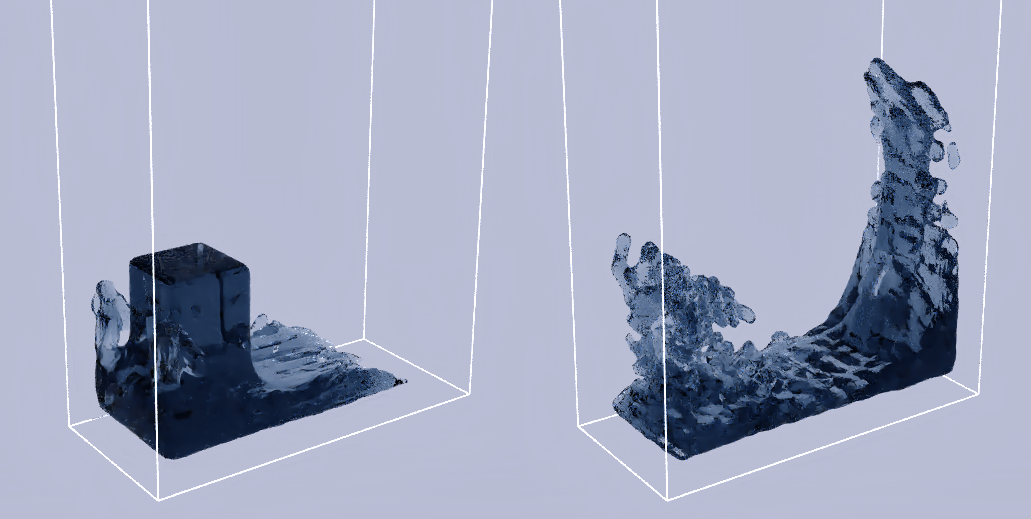
\includegraphics[width=.6\textwidth]{pics/surface.png}
    \caption{The outlook of our fluid volume after surface construction.}
    \label{fig:surface}
\end{figure}

\section{Particle Update}
\label{sec3}

We implement particle update solvers for weakly compressible SPH and position-based fluids separately.

\subsection{Weakly Compressible SPH}

In weakly compressible SPH, physical properties of fluid particles are updated through an array of explicit state equations. Fluid particles move around as a result of inter-particle interactions and external forces that act upon them. An outline of a single WC-SPH update is shown in Alg. \ref{alg1}. At the beginning of such an update step, a neighborhood search is carried out to determine the spatial neighbors of each fluid particle. Fluid and solid particle neighbors are stored separately to facilitate instant evaluation of function values at discrete locations in the fluid domain, which in the context of WC-SPH takes the form of an interpolation. Then, the fluid particle densities are estimated as they will be needed for the computation of interaction forces. As a logical next step, the incurred forces are evaluated for each particle and the resultant accelerations are accumulated for time integration.

\medskip
\begin{algorithm}[H]
	\DontPrintSemicolon
	\SetAlgoLined
	\SetAlgorithmName{Algorithm}{Algorithm}{List of Algorithms}
	\SetAlCapNameSty{textbf}
	\caption{\label{alg1} A Single WC-SPH Update}
	\SetKwFunction{FMain}{update}
	\SetKwProg{Fn}{Function}{:}{}
	\Fn{\FMain{$ \Delta t $}}{
		\For{each particle i}{
			find neighbors j\;
		}
		\For{each particle i}{
			compute density $ \rho_{i} $\;
		}
		\For{each particle i}{
			accumulate acceleration $ \boldsymbol{a}_{i} $ as a result of various component forces\;
		}
		\For{each particle i}{
			compute velocity at next time stamp $ \boldsymbol{v}_{i}\left(t + \Delta t\right) $\;
			compute position at next time stamp $ \boldsymbol{x}_{i}\left(t + \Delta t\right) $\;
		}
	}
\end{algorithm}
\medskip

Rather than to enforce strict incompressibility throughout the fluid domain, WC-SPH solvers allow a minor amount of volume compression to happen at every time step. Under such circumstances, per-particle density estimation in densely resided regions in the fluid domain would exhibit a deviation from the rest density of the fluid. As a consequence, we may observe considerable variances at discrete particle locations in the pressure field. To counteract such variances, a pressure force $ \mathbf{F}_{i}^{p} $ in the opposite direction to the spatial gradient of the pressure field is then generated for each particle. An evaluation of the pressure field at the discrete particle location $ \boldsymbol{x}_{i} $ may look like:

\begin{equation}
	\label{eq14}
    p_{i} = \max(0, \kappa(\rho_{i} - \rho_{0}))
\end{equation}

where $ \kappa $ is an artificial hyperparam that refers to the stiffness of the fluid. Negative pressure values are clamped to zero out of the practical concern to avoid clotting behaviour where particle neighborhoods are under-populated. 

In addition to pressure forces, typically viscosity forces $ \mathbf{F}_{i}^{v} $ and friction forces $ \mathbf{F}_{i}^{f} $ are also introduced to facilitate visually realistic fluid simulations. Viscosity forces counteract the divergence of the velocity field in the local space and lead to rather similar velocities for adjacent fluid particles. Friction forces, on the other hand, model the deceleration experienced by fluid particles that interact with static solid particles in the boundary. With such forces applied, we may accumulate the acceleration $ \boldsymbol{a}_{i} $ of a particle $ i $ as:

\begin{equation}
	\label{eq15}
	\boldsymbol{a}_{i} = \left(\mathbf{F}_{i}^{p} + \mathbf{F}_{i}^{e} + \nu \cdot \mathbf{F}_{i}^{v} + \mu \cdot \mathbf{F}_{i}^{f} \right) / M_{0}
\end{equation}

where $ \mathbf{F}_{i}^{e} $ represents external forces (typically gravity) and $ \nu $ and $ \mu $ are artificial hyperparams used to weight the respective components. We conduct ablation studies in Sec. \ref{sec4} to understand the effects of the aforementioned hyperparams.

\subsection{Position-based Fluids}

Instead of introducing an artificial pressure force to counteract density deviation, position-based fluids (PBF) pose a scalar constraint $ C_{i} $ on the estimated density of each fluid particle $ i $:

\begin{equation}
	\label{eq20}
	C_{i}(\hat{\boldsymbol{x}}) = \frac{\rho_{i}(\hat{\boldsymbol{x}})}{\rho_{0}} - 1 = 0
\end{equation}

\medskip
\begin{algorithm}[H]
	\DontPrintSemicolon
	\SetAlgoLined
	\SetAlgorithmName{Algorithm}{Algorithm}{List of Algorithms}
	\SetAlCapNameSty{textbf}
	\caption{\label{alg3} A Single PBF Update}
	\SetKwFunction{FMain}{update}
	\SetKwProg{Fn}{Function}{:}{}
	\Fn{\FMain{$ \Delta t $}}{
		\For{each particle i}{
			compute density $ \rho_{i} $\;
		}
		\For{each particle i}{
			accumulate acceleration $ \boldsymbol{a}_{i} $ as a result of various component forces\;
		}
		\For{each particle i}{
			compute velocity at next time stamp $ \boldsymbol{v}_{i}\left(t + \Delta t\right) $\;
			store old position $ \bar{\boldsymbol{x}}_i $\;
			compute position at next time stamp $ \boldsymbol{x}_{i}\left(t + \Delta t\right) $\;
		}
		\For{each particle i}{
			find neighbors j\;
		}
		\For{each iteration $ r \leq R $}{
			\For{each particle i}{
				compute density $ \rho_{i} $\;
				compute density constraint violation $ C_{i} $\;
				compute expression $ S_{i} $\;
				compute position correction stride $ \lambda_{i} $\;
			}
			\For{each particle i}{
				compute position correction $ \Delta \boldsymbol{x}_{i} $\;
				correct position $ \boldsymbol{x}_{i} $\;
			}
		}
		\For{each particle i}{
			update velocity $ \boldsymbol{v}_{i} $ from old position $ \bar{\boldsymbol{x}}_{i} $\;
		}
	}
\end{algorithm}
\medskip

where $ \hat{\boldsymbol{x}} $ denotes the concatenation of all position vectors involved in the computation of $ \rho_{i} $. The fulfillment of such a constraint implies that the fluid is largely at rest state in the local neighborhood and that the density of the respective particle lies roughly around $ \rho_{0} $. Under circumstances where such a constraint is violated, however, the solver seeks to find, in a Newton-like iterative manner, a position correction $ \Delta \hat{\boldsymbol{x}} $ that would locally restore the system to the rest state:

\begin{equation}
	\label{eq21}
	C_{i}(\hat{\boldsymbol{x}} + \Delta \hat{\boldsymbol{x}}) = 0
\end{equation}

An outline of a single PBF update is shown in Alg. \ref{alg3}. In each time step, accelerations that result from a range of internal and external forces are evaluated and then used to perform one time integration step. Then, the violation of the density constraint is determined for each particle. Out of the need to enforce volume conservation, we compute a position correction $ \Delta \hat{\boldsymbol{x}} $ that lies in the opposite direction as the spatial gradient of the constraint $ \nabla C_{i} $:

\begin{equation}
	\label{eq22}
	\Delta \hat{\boldsymbol{x}} = M^{-1} \nabla C_{i} \cdot \lambda_{i}
\end{equation}

where $ \lambda_{i} $ is the single variable that controls the stride of the correction. By pulling Eq. \eqref{eq22} into the first-order Taylor expansion of Eq. \eqref{eq21} we obtain:

\begin{equation}
	\label{eq23}
	C_{i}(\hat{\boldsymbol{x}}) + (\nabla C_{i})^{T} \Delta \hat{\boldsymbol{x}} = C_{i}(\hat{\boldsymbol{x}}) + (\nabla C_{i})^{T} M^{-1} \nabla C_{i} \cdot \lambda_{i} = 0
\end{equation}

As a logical next step we may compute $ \lambda_{i} $ as

\begin{equation}
	\label{eq24}
	\lambda_{i} = - \frac{\sigma \cdot C_{i}(\hat{\boldsymbol{x}})}{S_{i} + \epsilon}.
\end{equation}

where

\begin{itemize}
    \item $ S_{i} = (\nabla C_{i})^{T} M^{-1} \nabla C_{i} $.
    \item $ \epsilon $ is a small value added for nummerical stability.
    \item $ \sigma $ is an artificial damper used to downscale the correction stride.
\end{itemize}

Since the we are practically reaching for the solution of a non-linear system of equations with a linear approach, this correction may be applied multiple times until the violation shrinks to an acceptable scale. We conduct ablation study on how the number $ R $ of corrective iterations and the introduction of the stride damper $ \sigma $ affect the behaviour of the fluid in Sec. \ref{sec4}.

\subsection{Surface Tension}

To allow our simulations to further impress, cohesion forces and adhesion forces are added to our implementation to model surface tension at microscopic level.

\paragraph{Cohesion Forces}

Cohesion forces model the interation between a pair of water molecules when they get close. The distance between the two molecules decide whether they attract or repel each other. Given a special kernel function $ W^{c} $, the cohesion force incurred by a fluid particle in our simulation may be approximated as:

\begin{equation}
	\label{eq25}
	\mathbf{F}_{i}^{c} = - \gamma m_{i} \sum_{j \in \mathcal{N}_{i}:j \in \mathcal{F}} m_j K_{ij} W^{c}(\norm{\mathbf{x}_{i} - \mathbf{x}_{j}}, H) \cdot \frac{\mathbf{x}_{i} - \mathbf{x}_{j}}{\norm{\mathbf{x}_{i} - \mathbf{x}_{j}}}
\end{equation}

where $ \gamma $ is a hyperparam that controls the scale and $ K_{ij} = \frac{\rho_{i} + \rho_{j}}{2\rho_{0}} $ is a normalizer that compensates for under-population in the local space. Since cohesion forces alone are in practice insufficient to guarantee a water-like fluid surface, we introduce an additional component $ \mathbf{F}_{i}^{n} $ that counteracts a high curvature by enforcing surface normals evaluated at adjacent particle locations to be similar:

\begin{equation}
	\label{eq26}
	\mathbf{F}_{i}^{n} = - \gamma m_{i} \sum_{j \in \mathcal{N}_{i}:j \in \mathcal{F}} K_{ij} (\mathbf{n}_{i} - \mathbf{n}_{j})
\end{equation}

where $ \mathbf{n}_{i} $ and $ \mathbf{n}_{j} $ are surface normals at particle locations $ \mathbf{x}_{i} $ and $ \mathbf{x}_{j} $ respectively. Such surface normals in the fluid domain may be computed as:

\begin{equation}
	\label{eq27}
	\mathbf{n}_{i} = H \sum_{j \in \mathcal{N}_{i}:j \in \mathcal{F}} \frac{m_{j}}{\rho_{j}} \nabla W_{ij}
\end{equation}

For particles on the fluid interface this normal vector points in the direction that is orthogonal to the fluid surface, whereas for interior particles its magnitude remains close to zero.

\paragraph{Adhesion Forces}

Adhesion forces model the attraction between a pair of fluid and solid molecules in close vicinity. Given a special kernel function $ W^{a} $, the adhesion force incurred by a fluid particle in our simulation may be computed as:

\begin{equation}
	\label{28}
	\mathbf{F}_{i}^{a} = - \beta m_{i} \sum_{k \in \mathcal{N}_{i}:k \in \mathcal{B}} V_{k} W^{a}(\norm{\mathbf{x}_{i} - \mathbf{x}_{k}}, H) \cdot \frac{\mathbf{x}_{i} - \mathbf{x}_{k}}{\norm{\mathbf{x}_{i} - \mathbf{x}_{k}}}
\end{equation}

where $ \beta $ is a hyperparam that controls the scale. Effects of the aforementioned hyperparams are discussed in Sec. \ref{sec4}.

\section{Experiments}
\label{sec4}

We carry out a wide range of experiments to study the effects of various hyperparams on the behaviour of fluid particles and of the fluid in general.

\subsection{Weakly Compressible SPH}

For weakly compressible SPH we fix the scale of our scene and conduct control experiments to test out how different values of pressure stiffness $ \kappa $, viscosity $ \nu $ and friction $ \nu$ would lead to different characteristics of the fluid. Our dam-break scene adopts the following configurations:

\begin{itemize}
    \item Fluid volume: $ 1m \times 5m \times 1m $
    \item Sampling distance: $ 0.1m $
    \item Maximum timestep: $ 10ms $
    \item Number of particles: $ 5000 $
    \item Gravity: $ 9.7m \cdot s^{-2} $
\end{itemize}

The selection of proper hyperparam values is sensitive to the domain size and sampling distance. For the aforementioned dam-break scene we find visually realistic simulations under the combination of $ \kappa = 100.0 $, $ \nu = 0.05 $ and $ \mu = 0.05 $. To tune the hyperparams for a general scene, such a combination could be adopted as a starter.

\subsubsection{Pressure Stiffness}

The stiffness coefficient $ \kappa $ is used to scale the pressure forces generated to counteract density deviation. When a low stiffness coefficient is applied, volume conservation fails to a large extent and some fluid particles leak through the container boundary since there is not enough pressure force to prevent such penetration. The estimated density in the bottom part of the fluid domain will significantly exceed the rest density of the fluid. On the other hand, when the stiffness value is set too high, the counteractive pressure forces are so intense that they will cause instant explosions upon even mild particle interactions.

\begin{figure}[h]
    \centering
    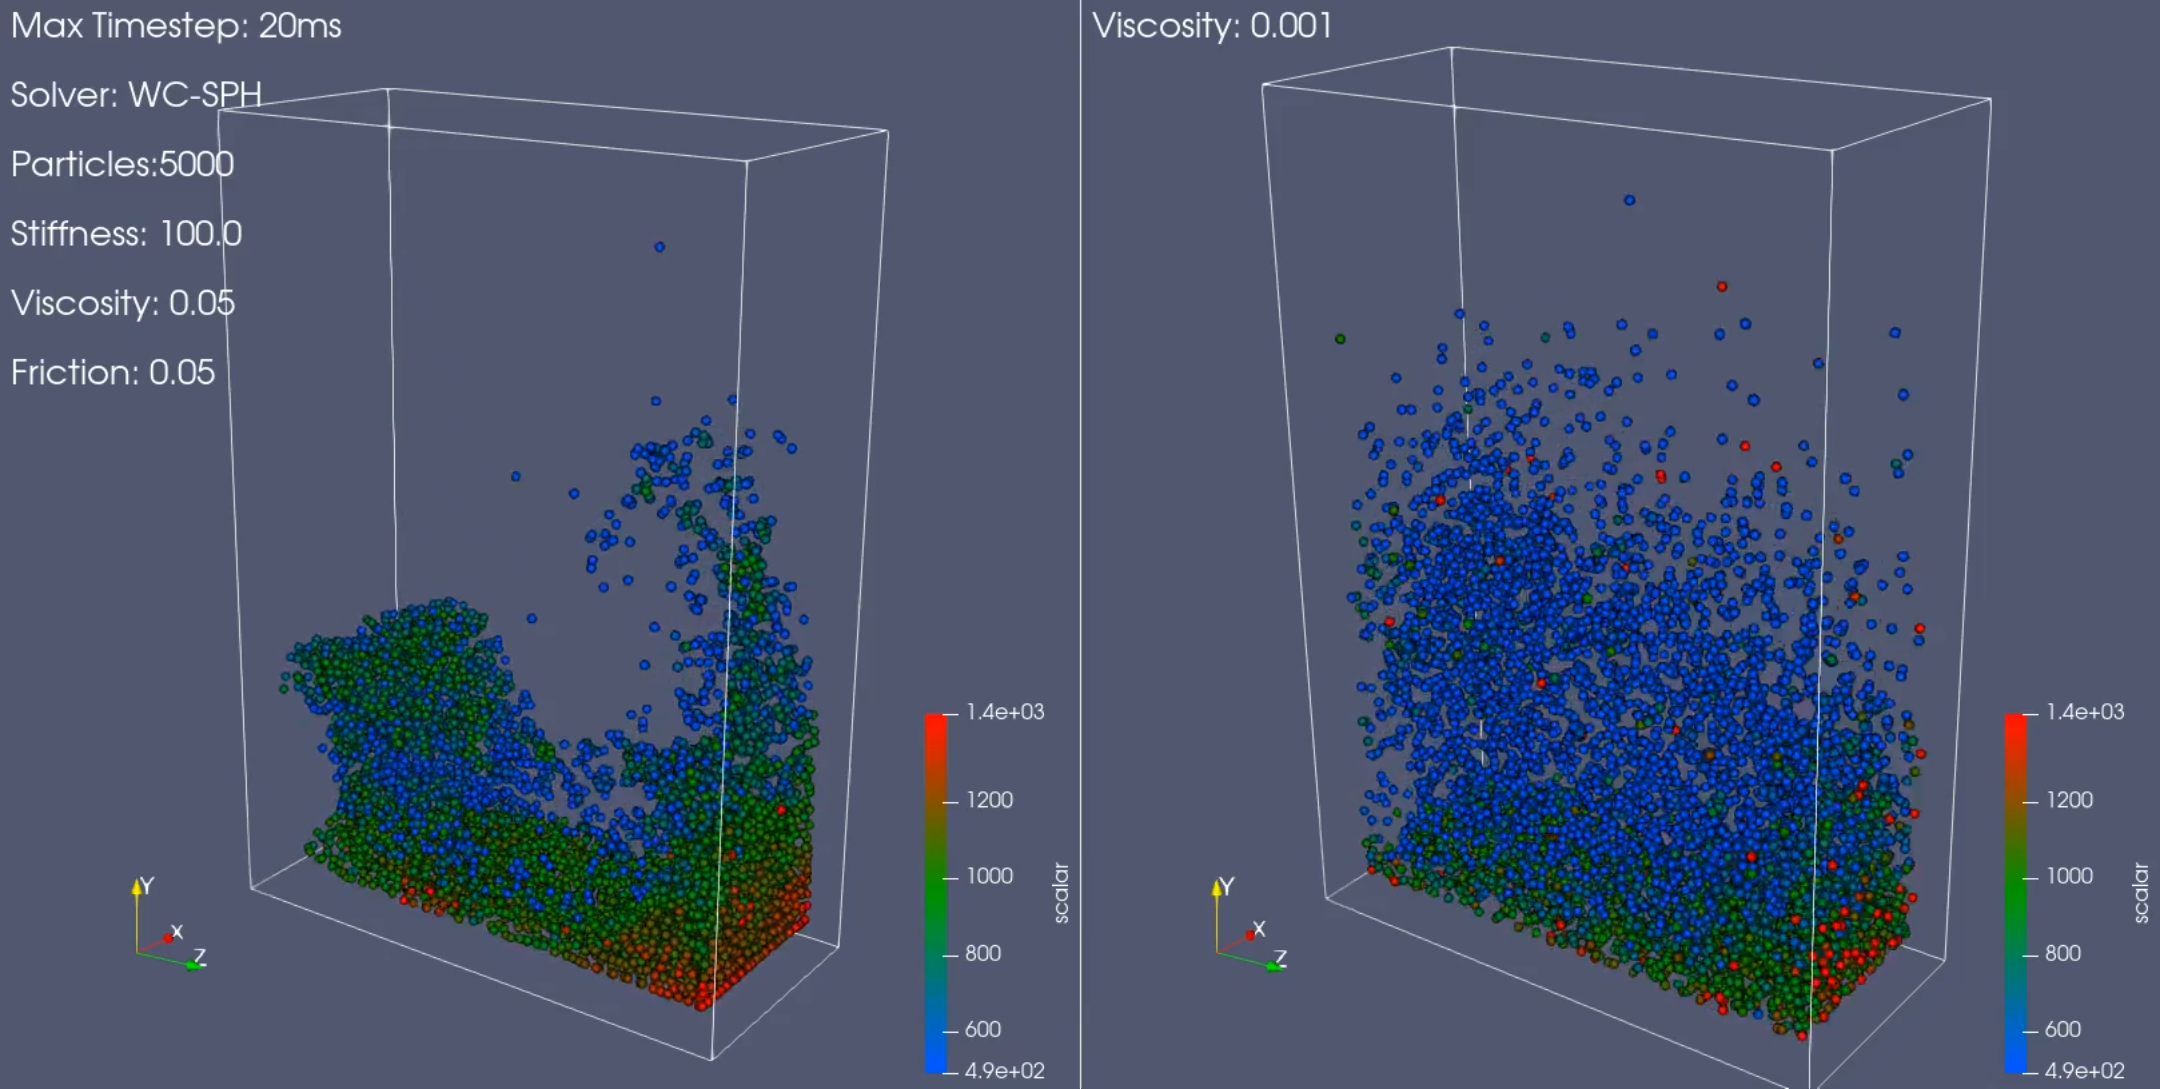
\includegraphics[width=.6\textwidth]{pics/wcsph_viscosity.png}
    \caption{Left: well-tuned simulation of a dam-break scene; Right: simulation of the same scene with rather low viscosity.}
    \label{fig:visco}
\end{figure}

\subsubsection{Viscosity}

The viscosity coefficient $ \nu $ is used to scale the tractive forces that acts inbetween fluid particles to model the viscous behaviour of the fluid. With such a force applied in a proper scale, the kinematic energy of a high-speed particle can be transferred to adjacent low-speed particles so that the divergence of the local velocity field is lessened and that the fluid particles end up moving as a whole locally. As can be observed in Fig. \ref{fig:visco}, however, too low a viscosity causes the fluid particles to behave rather like randomly bouncing molecules. This implies that the application of viscosity forces indeed dampens the energy of the system as a side effect.

\begin{figure}[h]
    \centering
    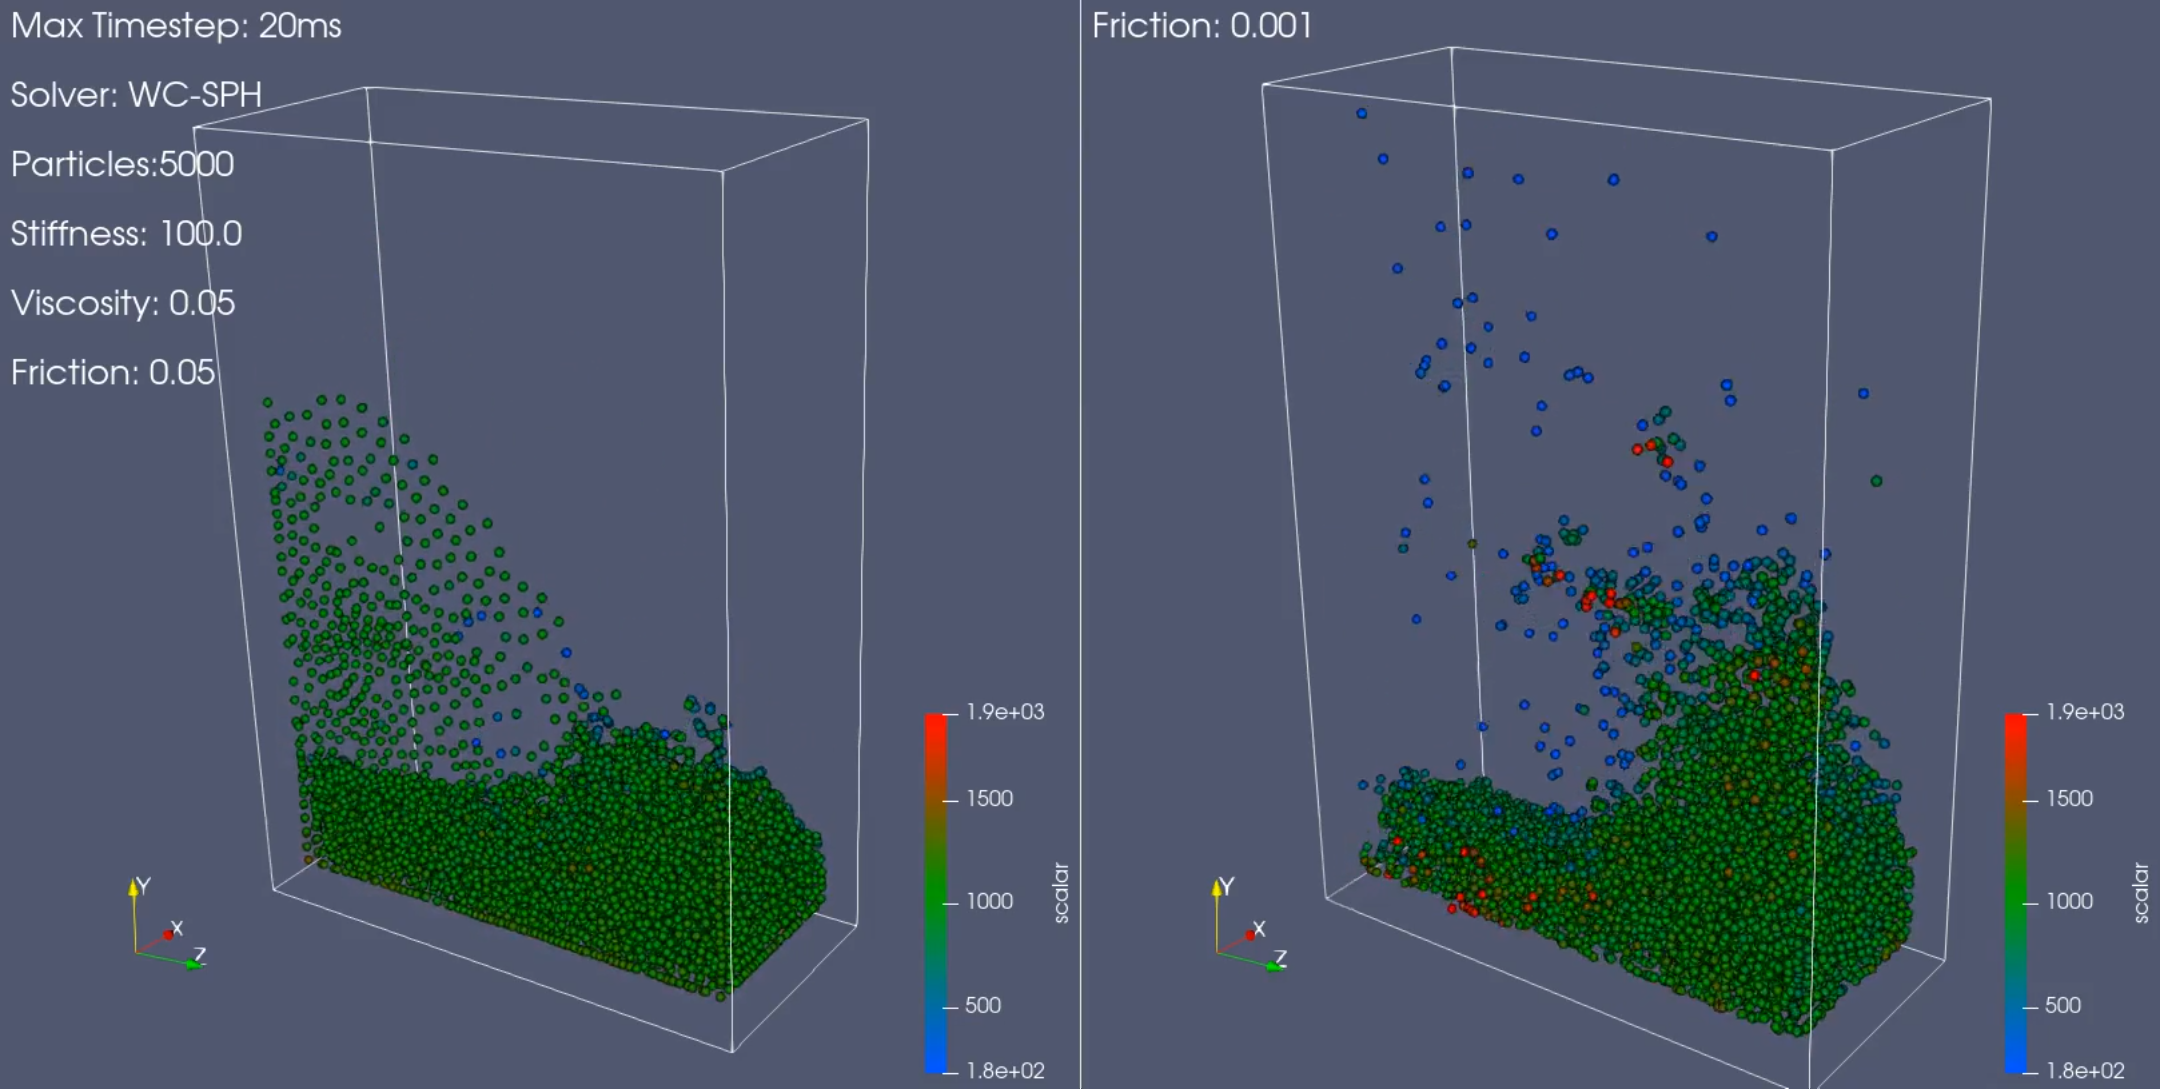
\includegraphics[width=.6\textwidth]{pics/wcsph_friction.png}
    \caption{Left: well-tuned simulation of a tipped dam-break scene; Right: simulation of the same scene with rather low friction.}
    \label{fig:frict}
\end{figure}

\subsubsection{Friction}

Similar to $ \nu $, the friction coefficient $ \mu $ is also used to scale a tractive force. What is different is that the latter controls the level of traction between fluid and solid particles. To easily demonstrate the effect of this hyperparam, we tip the container and the fluid cube by a 45-degree angle as an initial configuration. As is shown in Fig. \ref{fig:frict}, with properly scaled friction forces the fluid particles flow down rather slowly along the slope. The same does not happen with a low friction.

\subsection{Position-based Fluids}

Compared to WC-SPH, position-based fluids are rather stable against changes in scene configurations. Particles in PBF generally tend to exhibit higher viscosity, so we apply lower viscosity and friction for our experiments in this section. What has more of an impact on PBF simulations is the number $ R $ of corrective iterations per physical update and the maximum time step $ T_{0} $ that is allowed in the simulation. In addition to dam-break, we introduce a range of new test scenes to allow for more interesting observations. For experiments in this section the scenes are configured as follows:

\begin{itemize}
    \item Sampling distance: $ 0.1m $
    \item Number of particles: 10000
    \item Gravity: $ 9.7m \cdot s^{-2} $
\end{itemize}

\subsubsection{Middle-Layer Explosion}

\begin{figure}
    \centering
    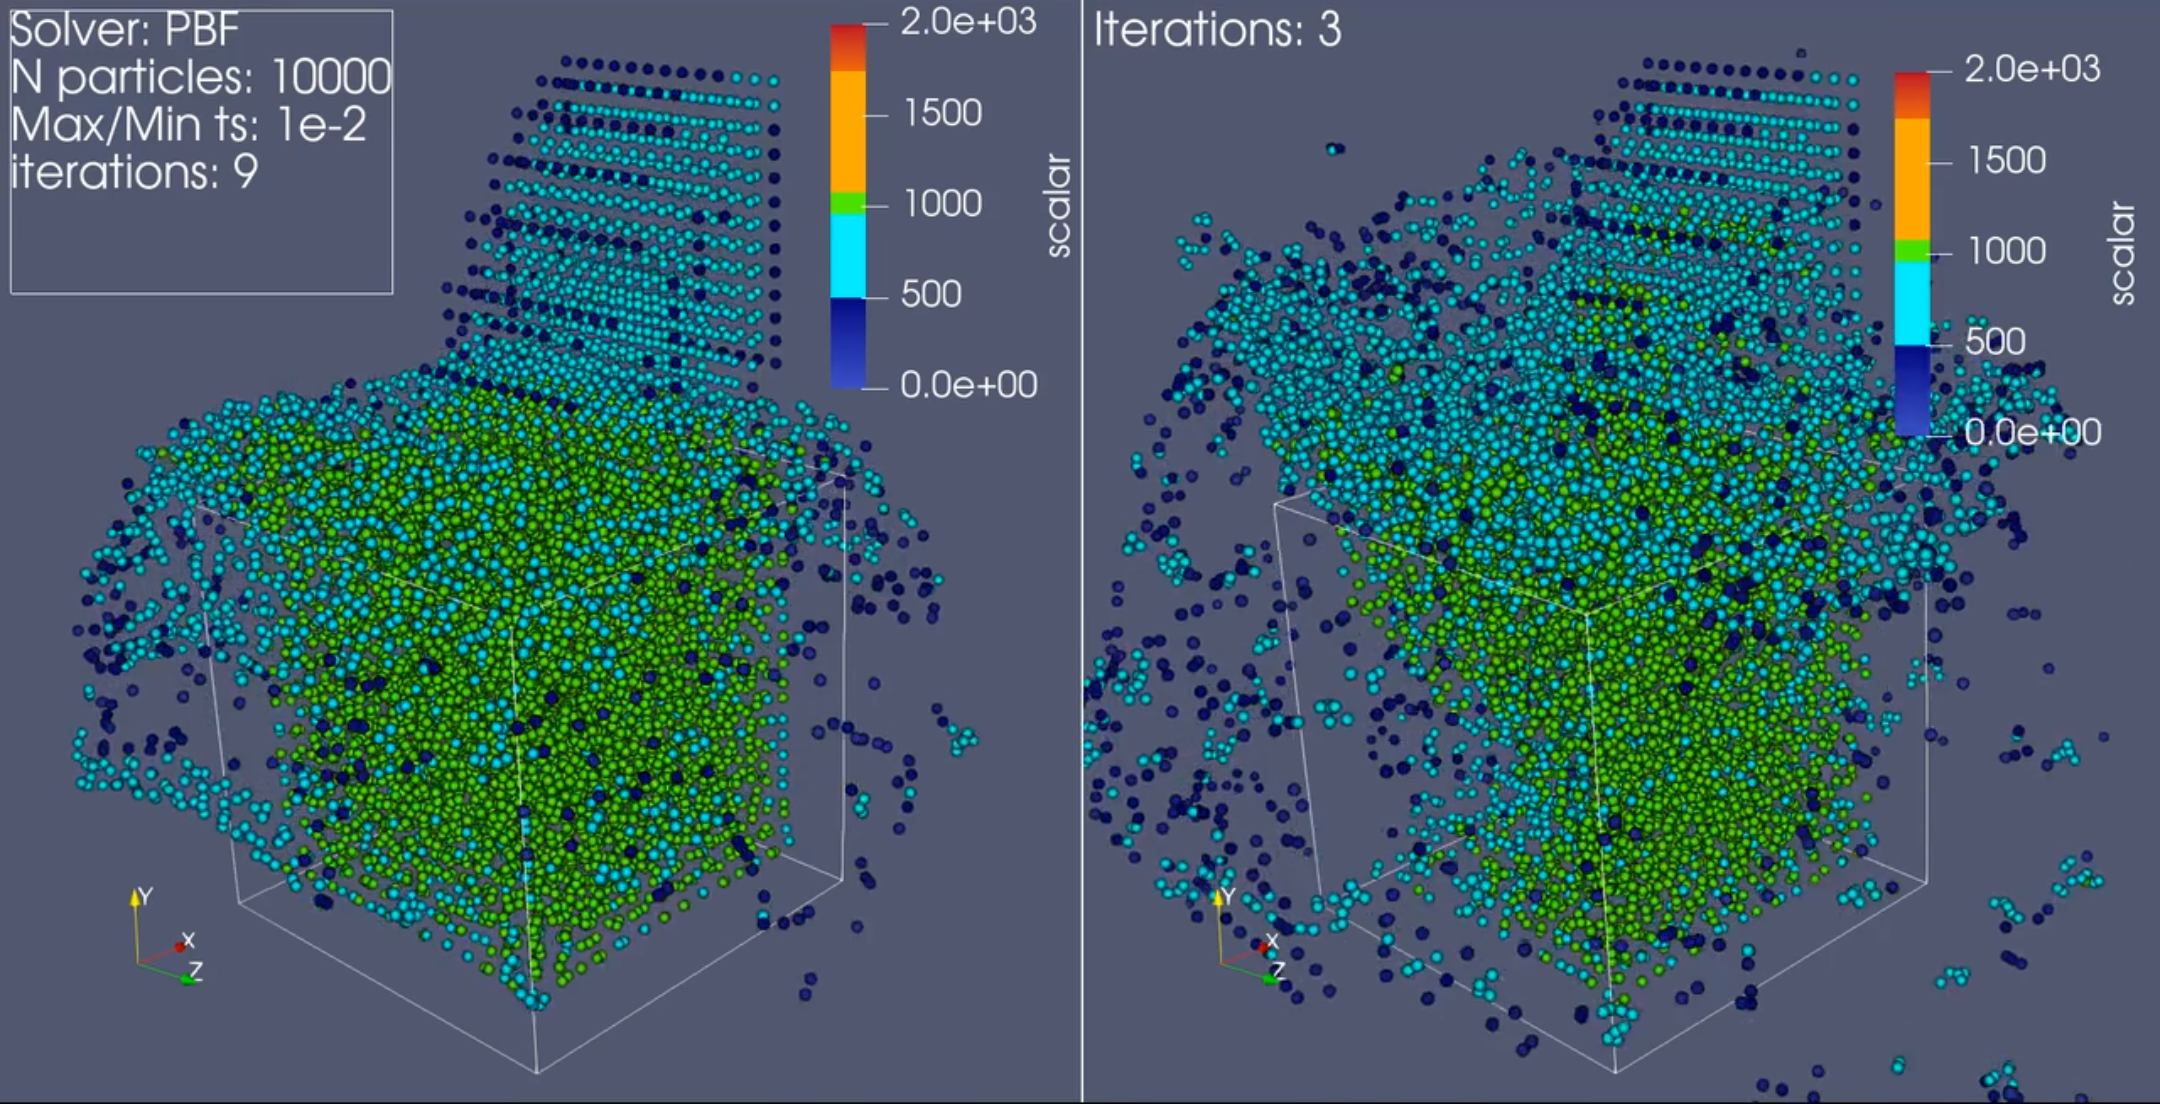
\includegraphics[width=.6\textwidth]{pics/pbf_iter.png}
    \caption{Left: well-tuned simulation of a box-fill scene; Right: simulation of the same scene with rather small number of corrective iterations.}
    \label{fig:boxfill}
\end{figure}

As we have observed in cases where we set a high time step cap and a low number of corrective iterations per physical update, a common problem for PBF is that the fluid volume tends to experience over pressure and explode from the middle every once in a while, especially when the fluid volume spans over a large depth range. As far as we can tell, such undesired behaviours follow from the fact that in many update steps the density constraints are under-fulfilled. Before the position correction, the over-pressured particles are those at the bottom of the fluid volume. With each corrective iteration, some particles in the lower layers of the fluid volume get transferred upwards, and as a result the pressure in the upper layers gradually rises. Given enough corrective iterations, the pressure experienced in the upper layers will be ultimately restored. However, when the correction procedure prematurely stops, over-pressure is still experienced somewhere in the middle of the fluid volume. Such over-pressure would accumulate over multiple update steps and eventually cause heavy explosions.

Fig. \ref{fig:boxfill} illustrates an example: With 9 corrective iterations per update, the fluid fills the container and then flow out of it smoothly after the container becomes full. With only 3 iterations, however, the fluid volume explodes roughly once every second. To solve this issue, we need to either apply smaller time steps or allow for more corrective iterations per update. According to the next set of experiments, taking the former option is a better choice.

\subsubsection{Double-Dam-Break}

We try out our PBF solver on a typical double-dam-break test scene with two different configurations as below:

\begin{itemize}
    \item $ T_{0} = 4ms $, $ \quad R = 8 $ iterations
    \item $ T_{0} = 2ms $, $ \quad R = 4 $ iterations
\end{itemize}

These two settings apply roughly the same number of corrective iterations for a fixed simulation length. As can be observed in Fig. \ref{fig:doubleDam}, with smaller time step cap and less iterations per update, we achieve arguably more realistic simulations and avoid minor explosions induced by over-pressure at the same time.

\begin{figure}[h]
    \centering
    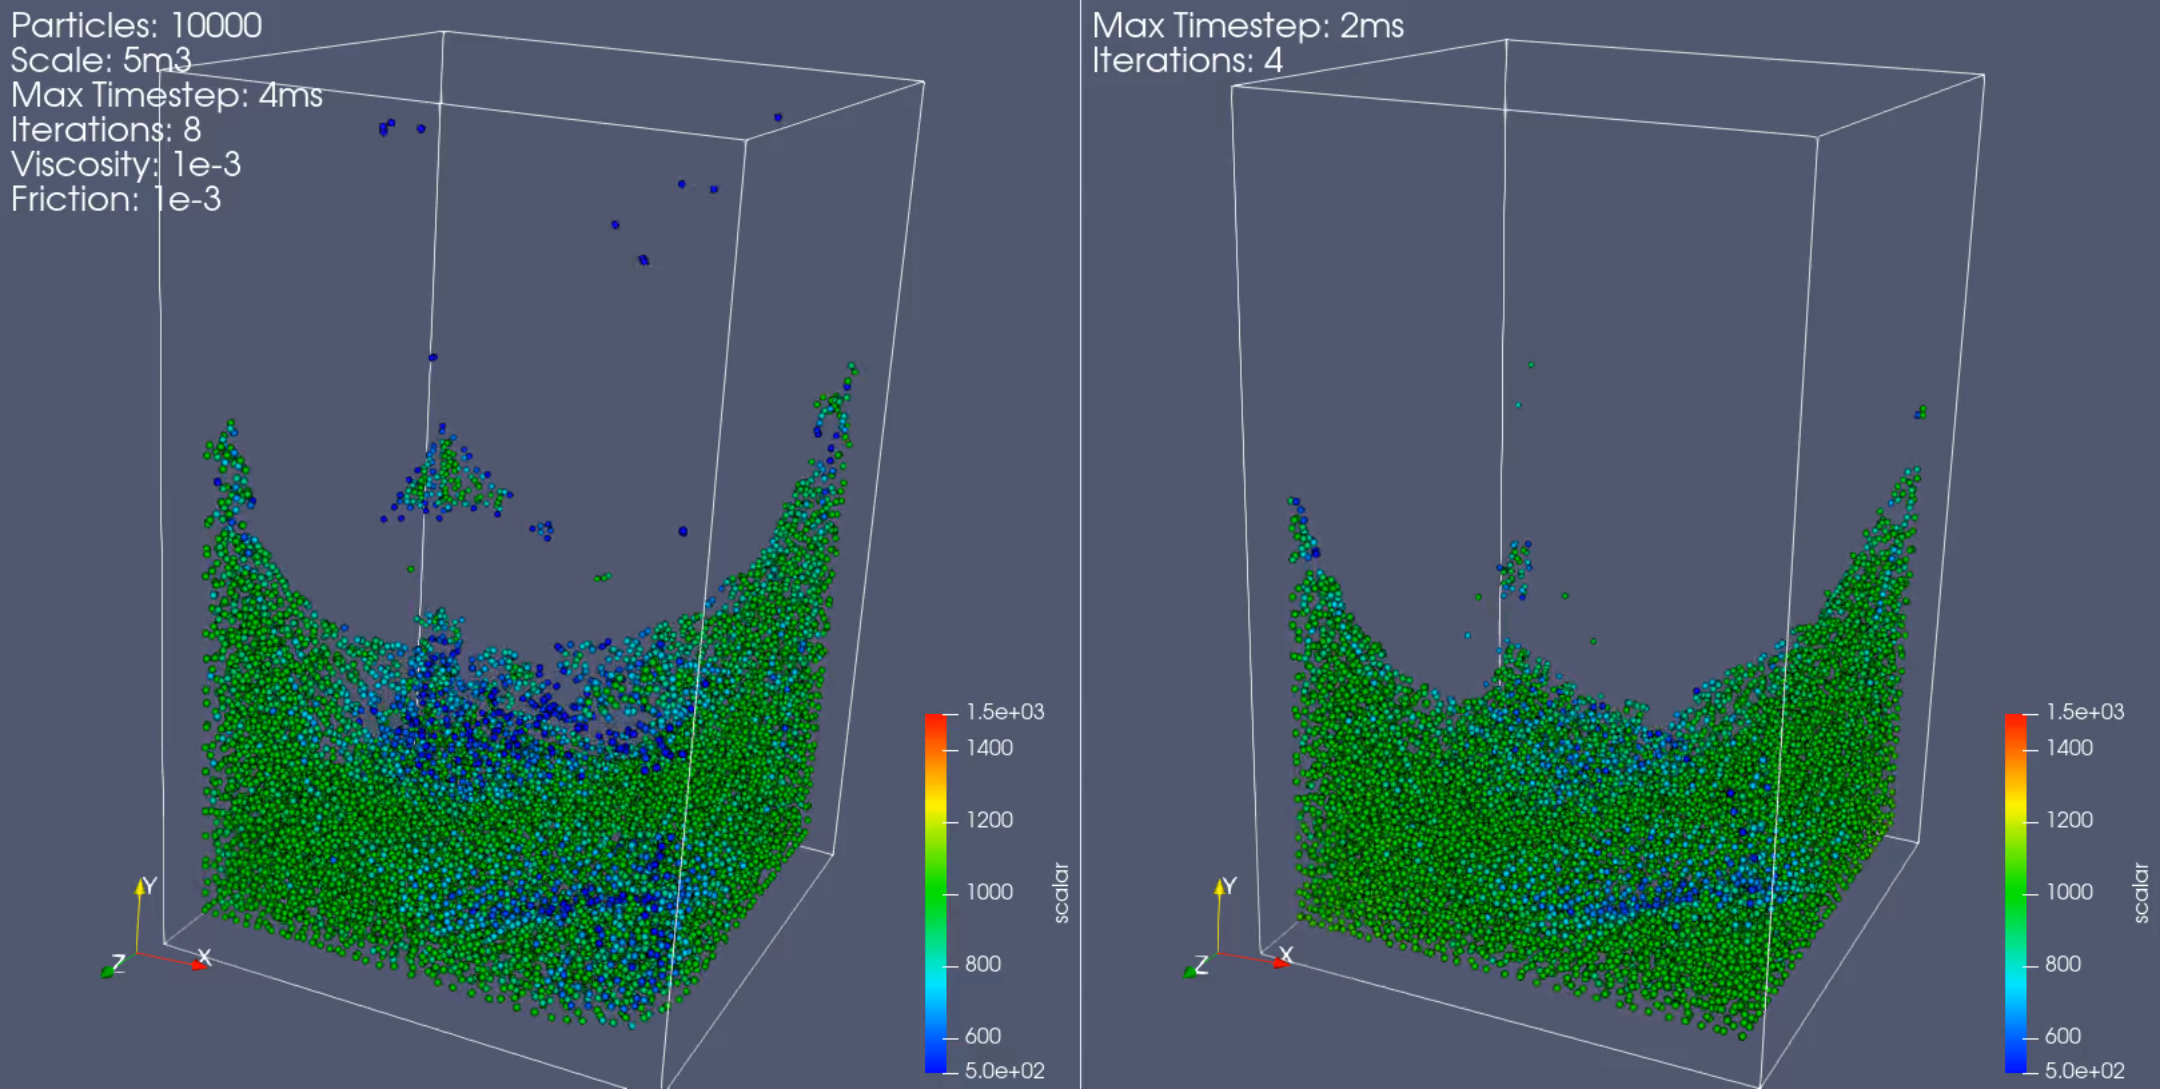
\includegraphics[width=.6\textwidth]{pics/pbf_iter_ts.png}
    \caption{Left: simulation of a double-dam-break scene with high $ T_{0} $ and large $ R $; Right: simulation of the same scene with low $ T_{0} $ and small $ R $.}
    \label{fig:doubleDam}
\end{figure}

\subsubsection{Stride Damper}

An alternative solution is to dampen the position correction stride with a small multiplier $ \sigma $. We try out our PBF solver on a typical dam-break scene with two different configurations as below:

\begin{itemize}
    \item $ T_{0} = 1ms $, $ \quad R = 3 $ iterations, $ \quad \sigma = 1.0 $
    \item $ T_{0} = 5ms $, $ \quad R = 3 $ iterations, $ \quad \sigma = 0.01 $
\end{itemize}

As is shown in Fig. \ref{fig:strideDamper}, both configurations yield visually acceptable results, with slight over-pressure at the bottom of the fluid volume noticable in the second simulation. But in terms of runtime, statistical analysis shows that the former one applies roughly 2.5 times as many corrective iterations as the latter one. Therefore we argue that the stride damper gives a good trade-off between visual plausibility and efficiency.

\begin{figure}[h]
    \centering
    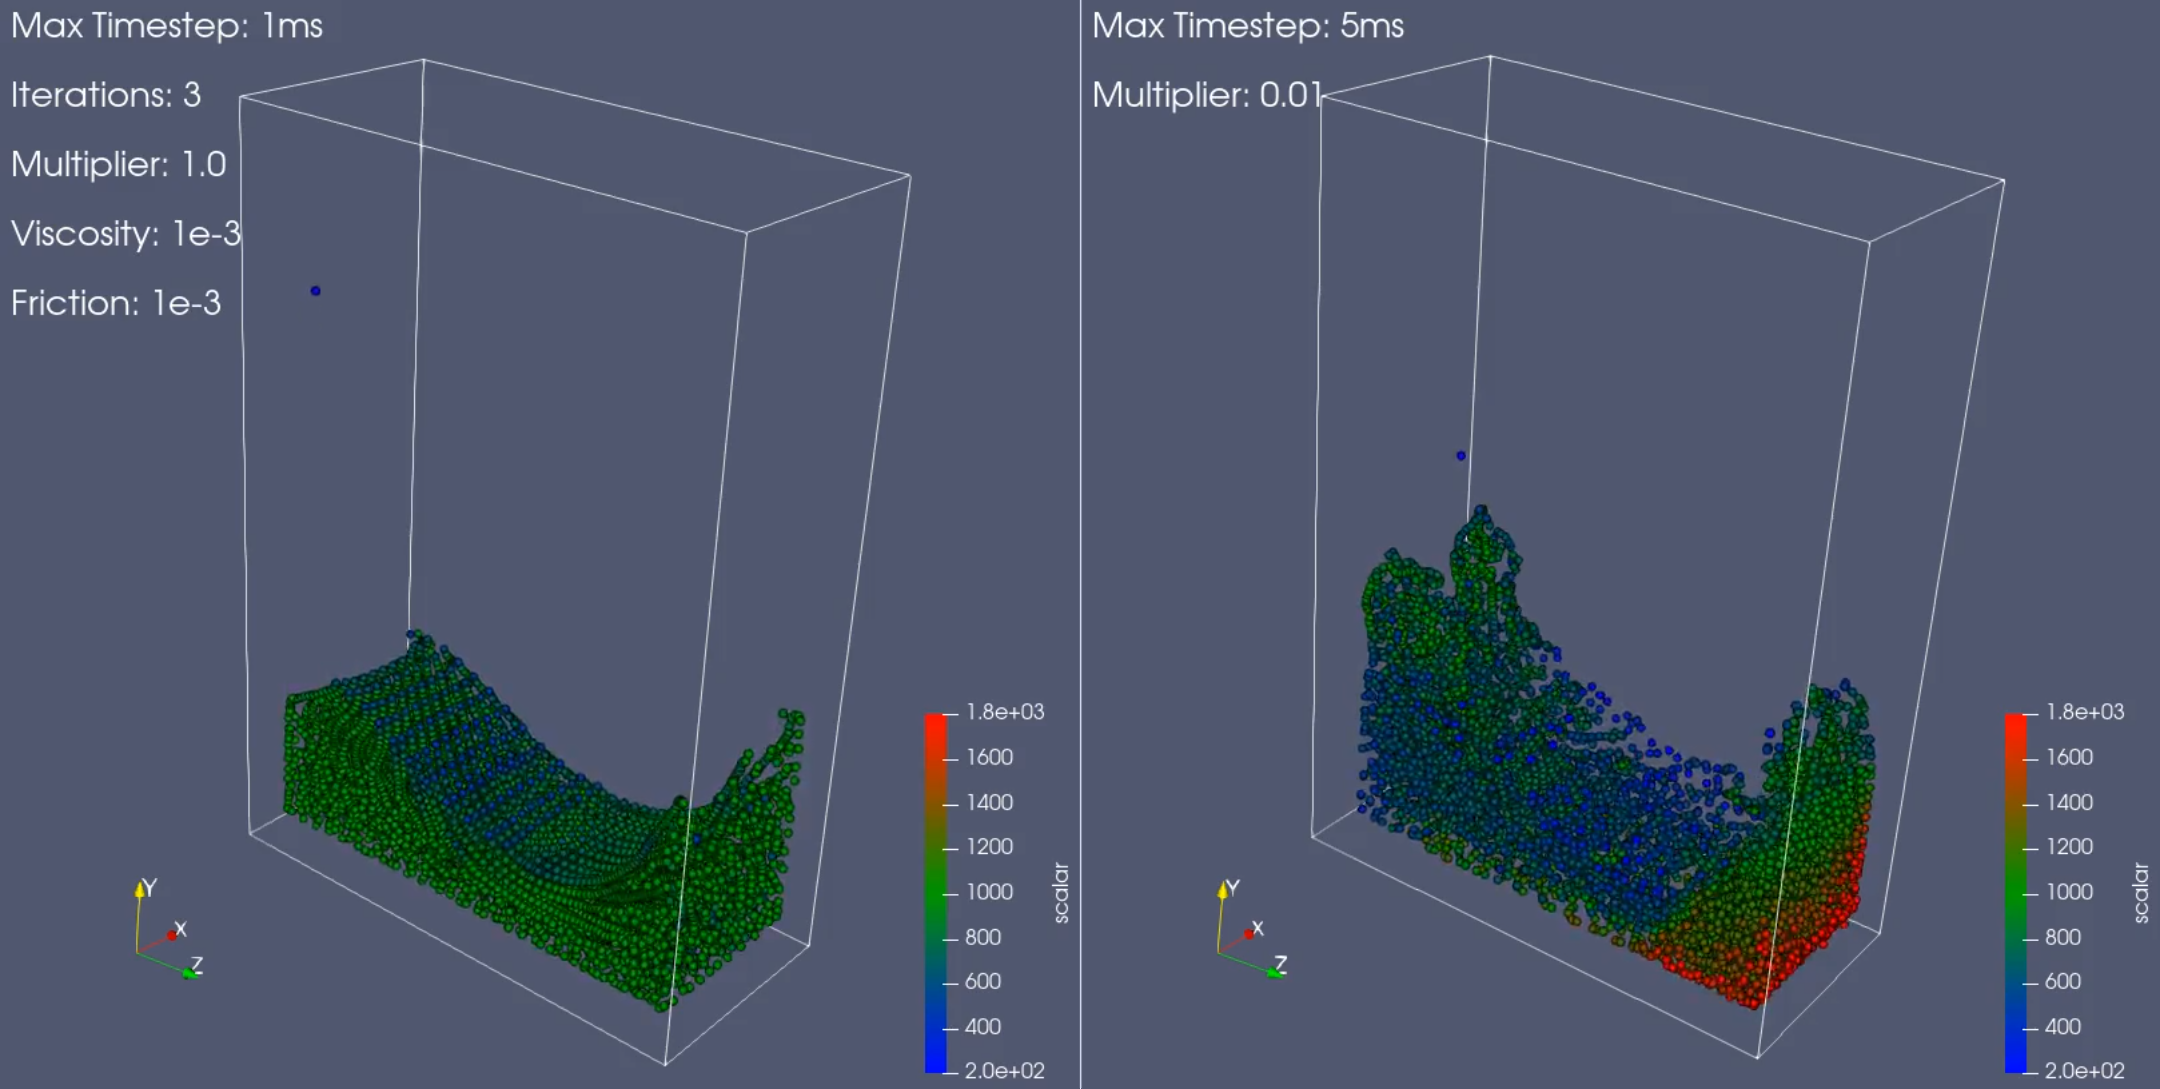
\includegraphics[width=.6\textwidth]{pics/pbf_stride_damper.png}
    \caption{Left: simulation of a dam-break scene with small $ T_{0} $; Right: simulation of the same scene with large $ T_{0} $ and the stride damper applied.}
    \label{fig:strideDamper}
\end{figure}

\subsection{Surface Tension}

In our simulations the scale of cohesion forces, i.e., attractive forces that act inbetween fluid particles, is controlled by $ \gamma $. The weight of adhesive forces, i.e., forces that model the tendency of fluid particles to attach to solid surfaces, is represented by $ \beta $. We conduct various control experiments to test out how different values of $ \gamma $ and $ \beta $ affect the fluid behaviour in terms of surface tension.

\begin{figure}[h]
    \centering
    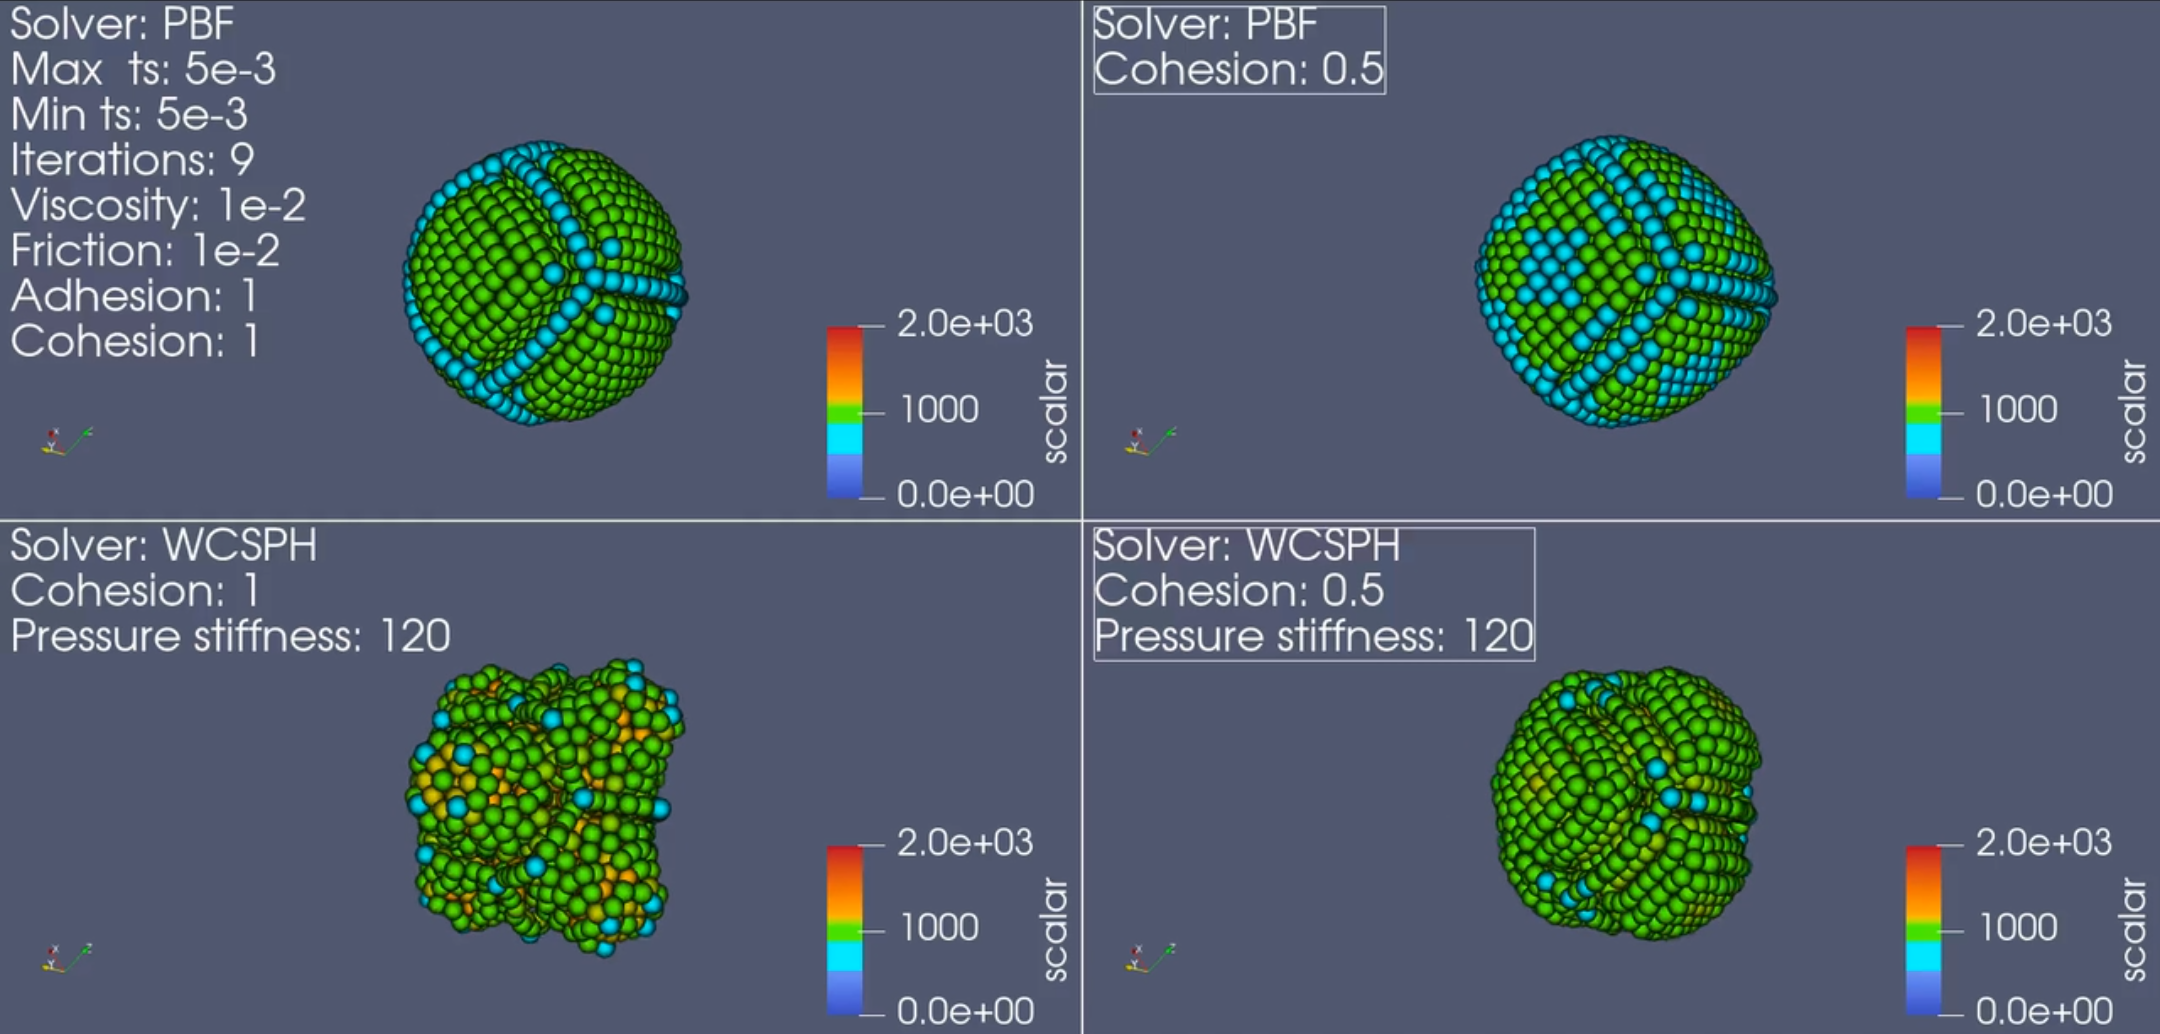
\includegraphics[width=.6\textwidth]{pics/surface_tension.png}
    \caption{Shape of fluid volume after half a second.}
    \label{fig:no_gravity}
\end{figure}

\subsubsection{Zero Gravity}

To verify how the choice of simulation solver affect surface tension in general, we place a fluid cube in the middle of the camera view and remove gravity to see how the outer surface of the fluid volume evolves with respect to time. We additionally test out how different values of $ \gamma $ affect the evolving process. As is shown in Fig. \ref{fig:no_gravity}, we may draw the following conclusions:

\begin{itemize}
    \item Under large $ \gamma $ values, convergence of the fluid cube to a perfect sphere is faster.
    \item Under small $ \gamma $ values, the WC-SPH solver suffers from oscillation in comparison.
\end{itemize}

\subsubsection{Wetting}

To verify how the choice of adhesion coefficient $ \beta $ may affect the fluid behaviour, we place a solid sphere under a particle generator that regularly emits fluid particles with a fixed intitial velocity, and observe how the fluid particles would attach to the sphere surface as they make contact. As can be observed in Fig. \ref{fig:wetting}, the higher the coefficient value, the stronger the attraction between fluid and solid particles. Depending on what type of fluid the user wants to model, the adhesion coefficient should empirically be selected from the range $ [1.0, 5.0] $.

\begin{figure}[h]
    \centering
    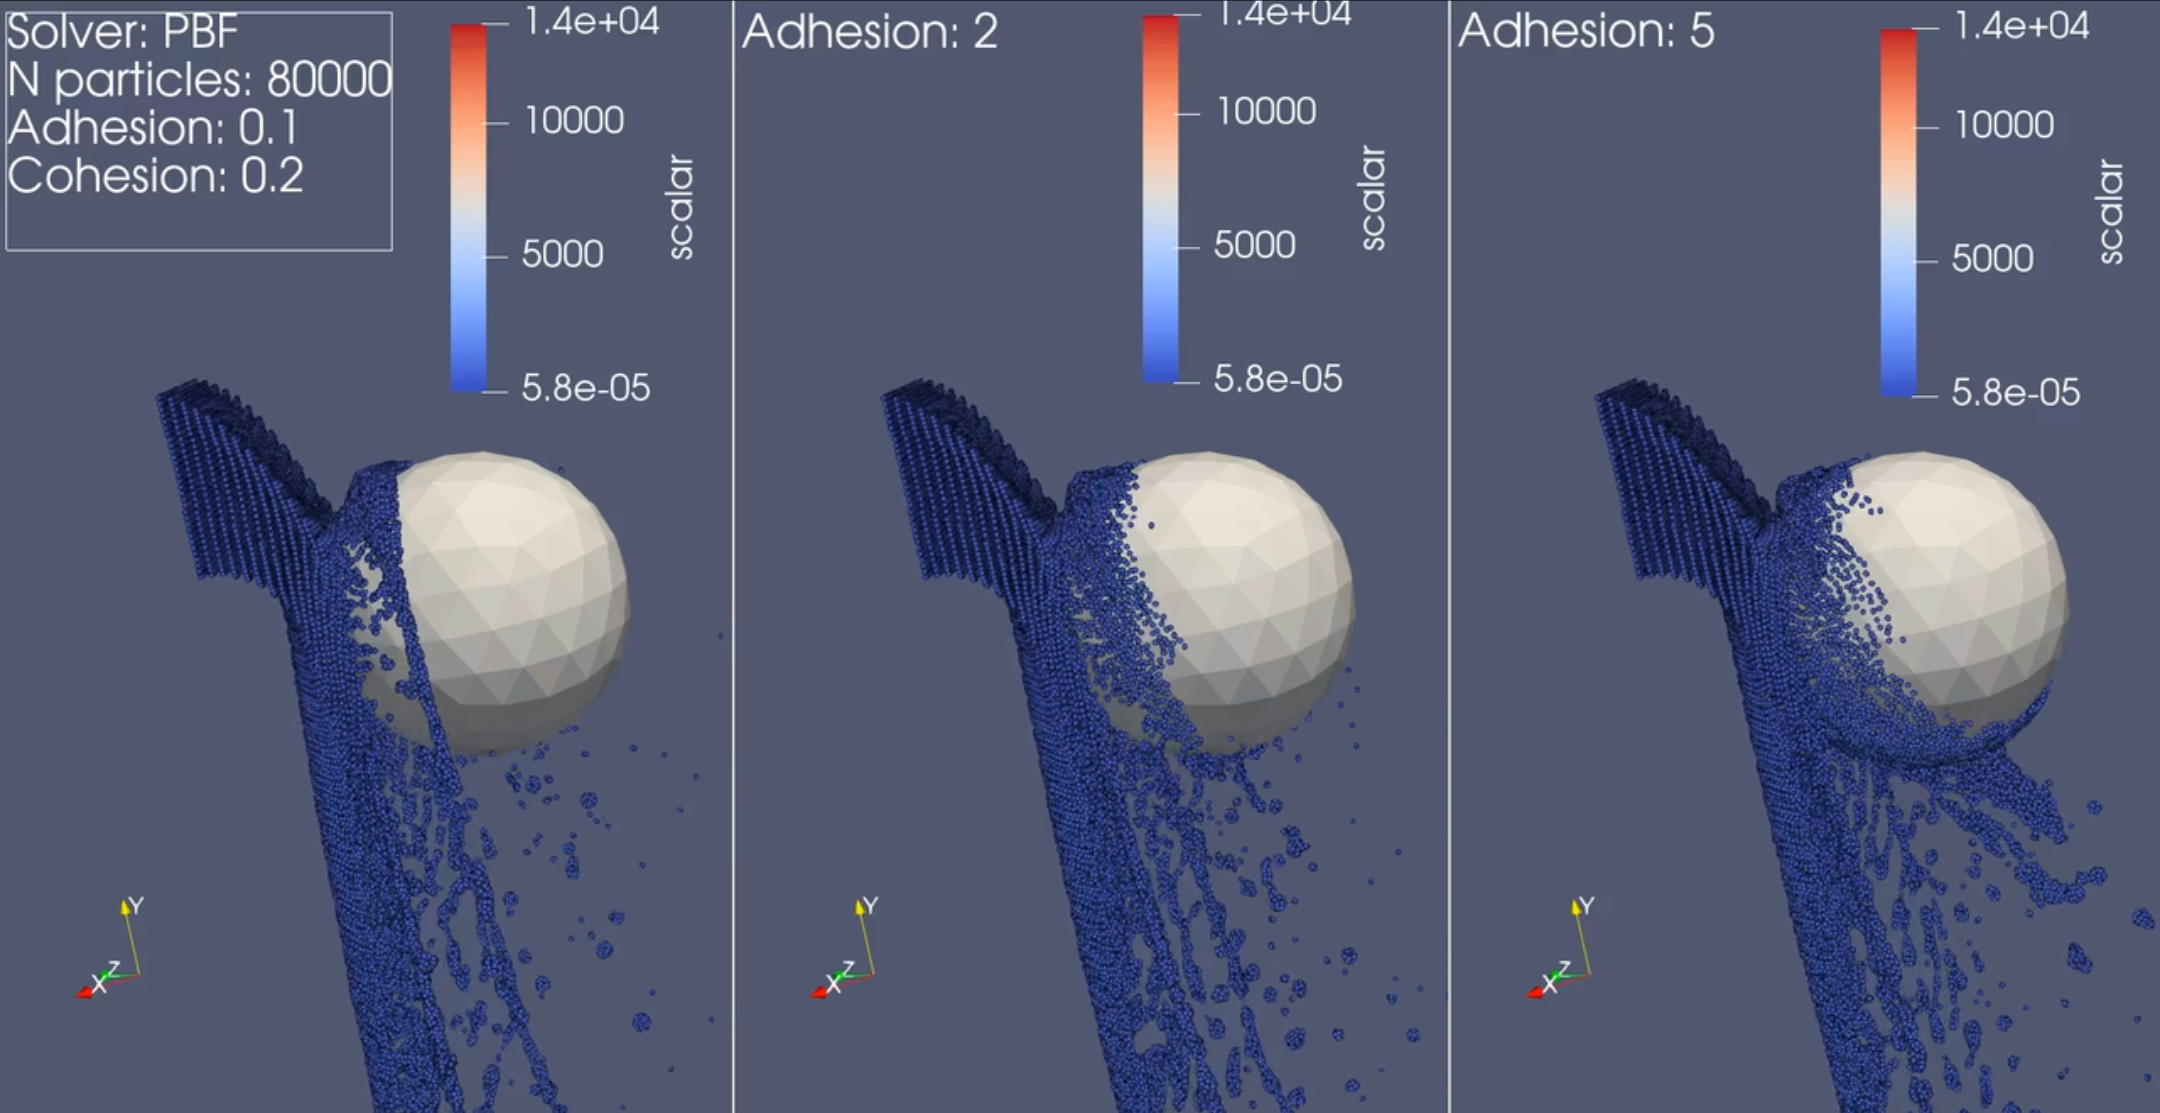
\includegraphics[width=.6\textwidth]{pics/adhesion.png}
    \caption{Wetting effect under different values of adhesion coefficient.}
    \label{fig:wetting}
\end{figure}

\begin{figure}[h]
	\centering
    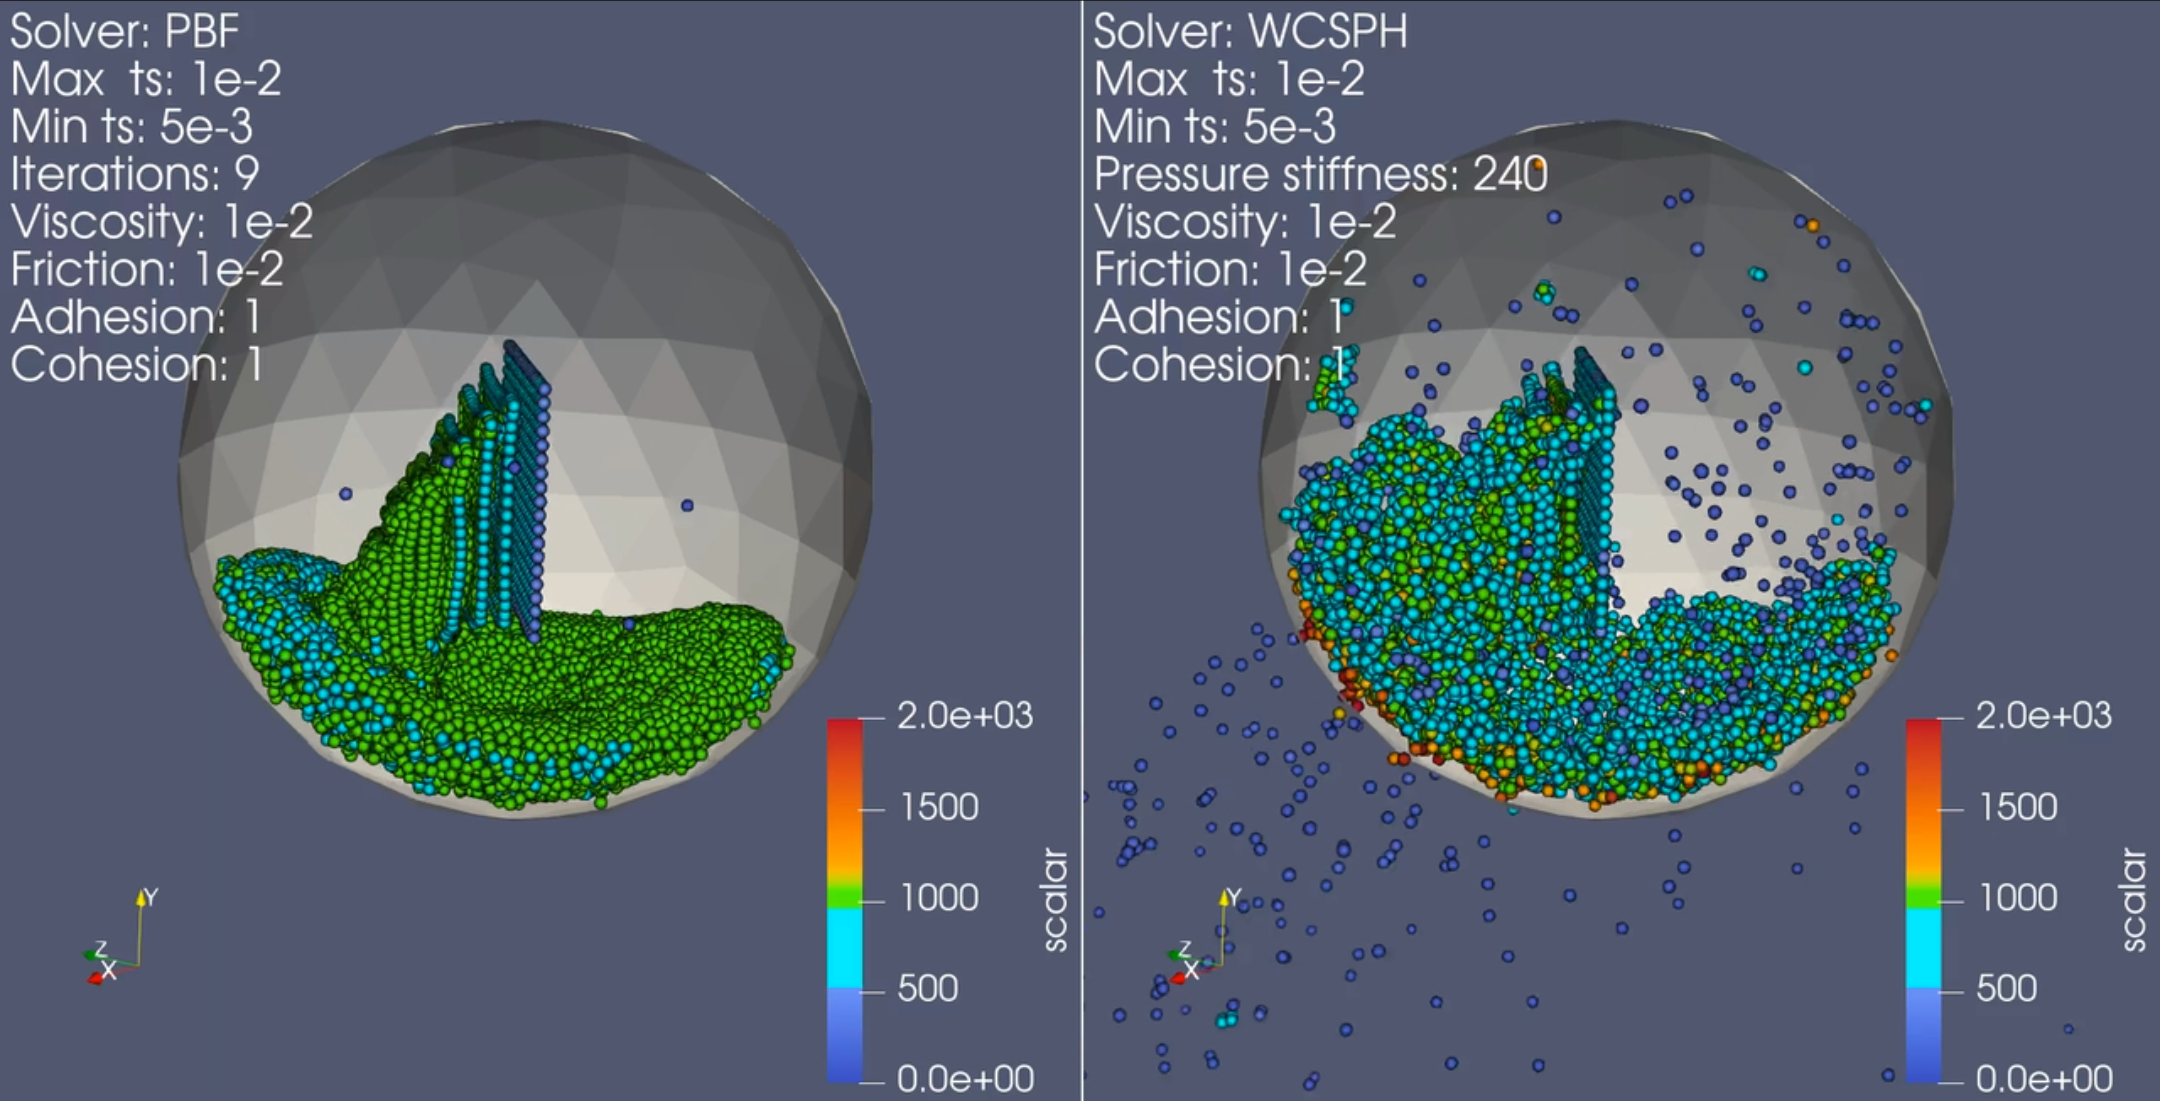
\includegraphics[width=.6\textwidth]{pics/comparison.png}
    \caption{Left: well-tuned simulation of a sphere-fill scene driven by PBF solver; Right: simulation of the same scene driven by WC-SPH solver under similar hyperparam settings.}
    \label{fig:comparison}
\end{figure}

\subsection{Comparison}

With an inherently different philosophy at its core, PBF solvers can entail very different outcomes compared to WC-SPH solvers even under similar scene configurations. To demonstrate this, we setup our solvers using a common hyperparam configuration that would suit both solvers under simple dam-break scenes, then place a particle emitter at the center of a spherical container to see how the fluid particles driven by different solvers would behave in general. As can be observed from Fig. \ref{fig:comparison}, the fluid particles in our PBF simulation demonstrate good stability even under heavy interactions. In contrast, in our WC-SPH simulation some particles leak out of the container due to insufficient pressure support, while some others bounce back heavily upon initial contact with the border. To summarize the differences, we list out below some key aspects of the PBF solver that is quite noticable:

\begin{itemize}
    \item PBF solvers demand typically much less of a tuning effort for new scenes.
    \item PBF solvers entail more viscous fluid behaviour in general.
    \item PBF solvers are better suited to scenes featuring intensive interactions.
\end{itemize}

However, the aforementioned merits of PBF solvers does not come without a price. To understand how both solvers behave in terms of their performance, we conduct (for a fixed dam-break scene) a quantitative analysis on how their runtime (under the assumption that both solvers manage to govern a stable simulation) grow with an increasing number of fluid particles. As can be observed in Fig. \ref{fig:performance}, the runtime of both solvers scale linearly with the number of particles and the PBF solver demands more time to handle the same number of particles. Considering a large part of the runtime for each update step is devoted to the neighborhood search, the actual performance gap is even higher than what is exhibited in the graph.

\begin{figure}[h]
	\centering
    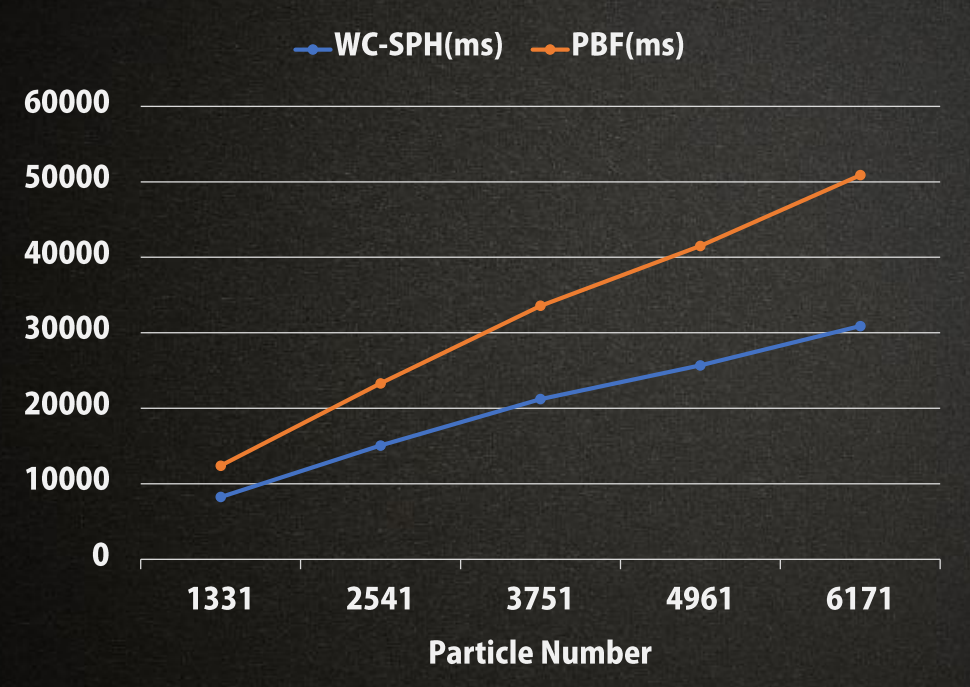
\includegraphics[width=.6\textwidth]{pics/performance.png}
    \caption{The runtime demanded by both solvers with respect to an increasing number of fluid particles in the simulation.}
    \label{fig:performance}
\end{figure}

\bibliographystyle{alpha}
\bibliography{references}

\end{document}
